\documentclass[fleqn, a4paper]{report}
\usepackage[top=1.5in,bottom=1.5in,left=1.15in,right=1.15in]{geometry}
\usepackage{graphicx}
\usepackage{tikz}
\usetikzlibrary{automata, positioning, arrows}
\usepackage[export]{adjustbox}
\usepackage{float}
\usepackage{gensymb}
\usepackage{amsmath}
\usepackage{booktabs}
\usepackage{tabularx}
\usepackage{lipsum}
\usepackage{pgfplots}
\usepackage{subfig}
\pgfplotsset{compat=1.15}
\usepackage[utf8]{inputenc}
\usepackage{hyperref}
\hypersetup{
    colorlinks=true,
    linkcolor=blue,
    filecolor=magenta,      
    urlcolor=cyan,
}

\title{EE463 Static Power Conversion I 
-Simulation Project III}
\author{Nail Tosun}
\date{November 2018}

\usepackage{natbib}
\usepackage{graphicx}

\begin{document}


\maketitle

\section*{Introduction}
In this simulation project, we investigated single phase and three phase controlled rectifier topologies. The differences, pros and cons of fully controlled and hald controlled single phase rectifier topologies discussed Q1. First part of the Q2 we used 3 phase full wave rectifier for driving DC motor. The speed, torque and armature current of rectifier investigated. We propose 2 methods for improving torque ripple. Then, the efficiency and components of power losses showed. Selection of diode and rectifier module be explained part 2. At Q3 we examined an alternative rectifier topology, 12 pulse rectifier, describe its operation and application areas and we showed the differences between full wave diode rectifier. 
\section*{Abbreviations}
\begin{table}[H]
\begin{tabular}{ll}
\textbf{THD} & Total Harmonic Distortion \\
\textbf{Qx}  & x'th question \\
\textbf{FFT} & Fast Fourier Transform\\
\textbf{PCC} & Point of Common Coupling \\
\textbf{l-l} & Line to Line \\
\textbf{pf} & Power Factor \\
\textbf{RMS} & Root Mean Square
\end{tabular}
\end{table}
\section*{Question 1}
\subsection*{3-Phase Thyristor Converter}
In this question, we are proposed 3 closed loop control topologies for speed regulation of DC motor drive. 
Characteristic of DC motor we used is following;
\begin{table}[H]
\centering
\begin{tabular}{ll}
\textbf{Field Type}          & Permanent Magnet    \\
\textbf{Armature Resistance} & $R_a = 10 \ohm$     \\
\textbf{Armature Inductance} & $L_a = 0.01 H$      \\
\textbf{Back-emf Constant}   & $0.3 \frac{V}{rpm}$ \\
\textbf{Motor Inertia}       & $0.4 kg m^2$       
\end{tabular}
\end{table}
The proposed methods are, 
 
\begin{itemize}
  \item On/Off Controller
  \item PI Controller
  \item Extended PI Controller with linearization
\end{itemize}
\subsubsection*{On/Off Controller}
The aim of the on/off controller is manipulating firing angle $0 \degree$ and $180 \degree$ for opening and closing the thyristor. The main advantages of on/off controller is it is simple, easy to implement and memoryless (no need external memory to store past error values).  We drive the controller with 50 Hz. The unit measure to error with 50 Hz sampling frequency and hold it through period. Depending on the error it fires thyristor $0 \degree$ an 180 $\degree$. 
The clear disadvantage of on-off controller is observed when steady-state occur. Since it can not do small changes at error signal, it oscillate around to steady state which called bang-bang. 
\begin{figure}[H]
    \centering
    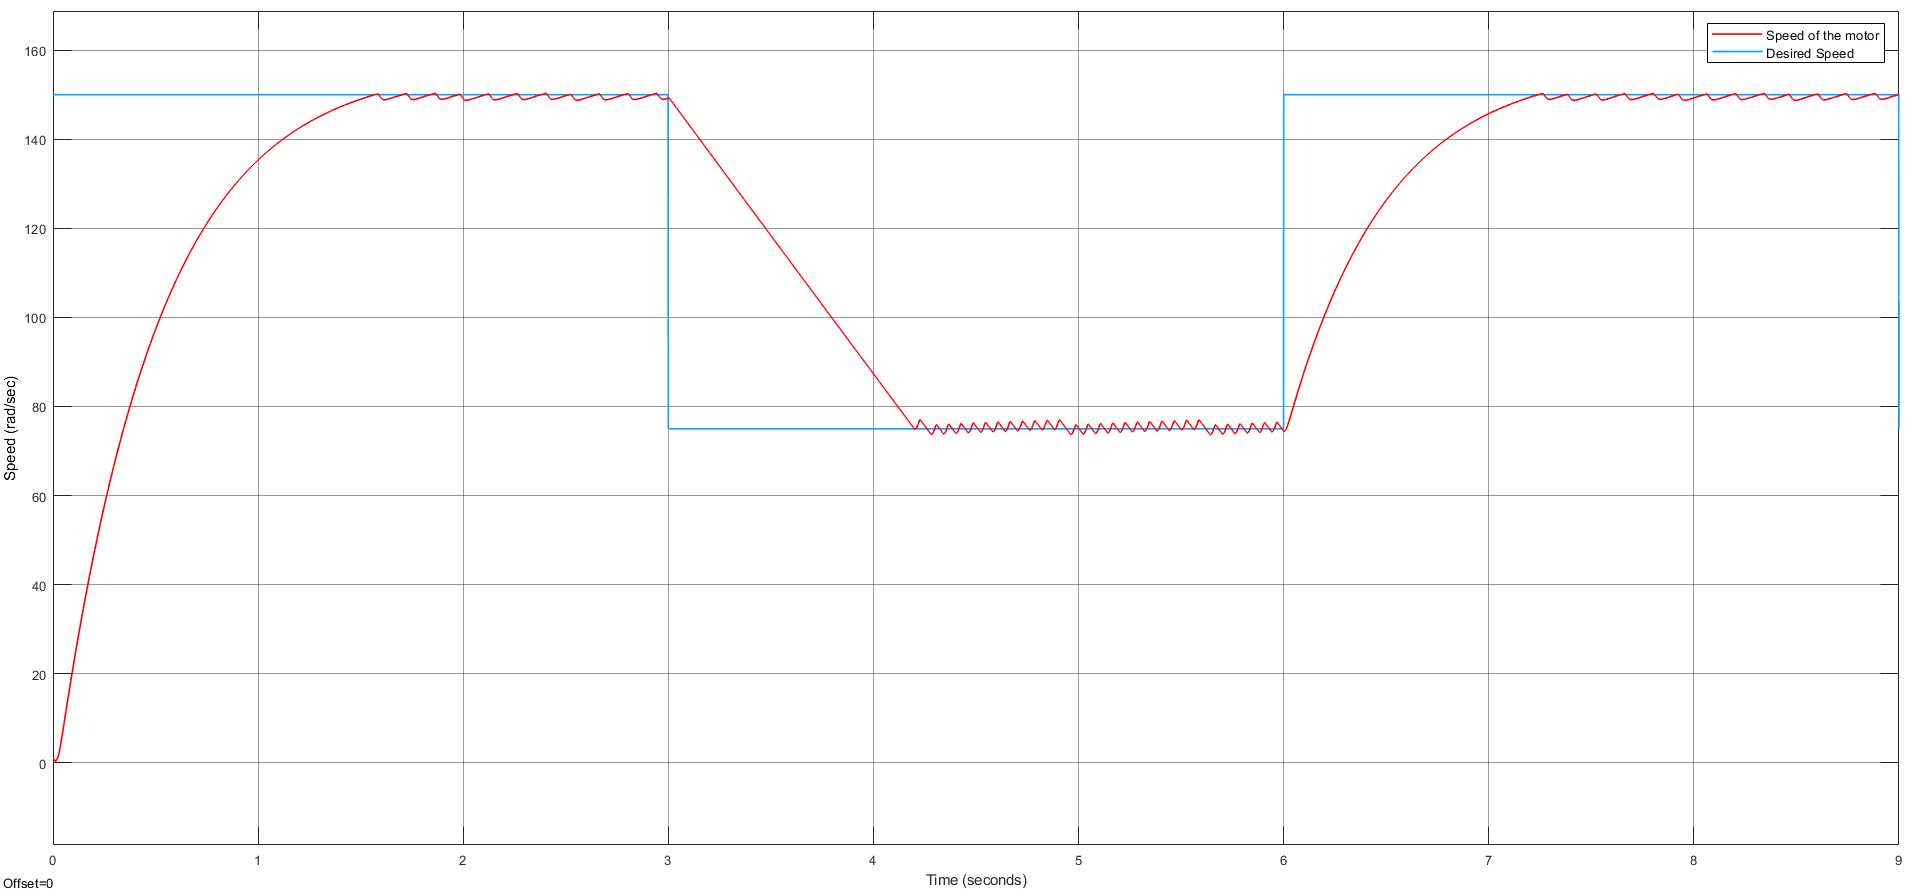
\includegraphics[width=10 cm]{on-off-controller.png}
    \caption{Transient speed response of the motor}
    \label{fig:my_label}
\end{figure}
This oscillations can be clearly seen by also from controller output. 
\begin{figure}[H]
    \centering
    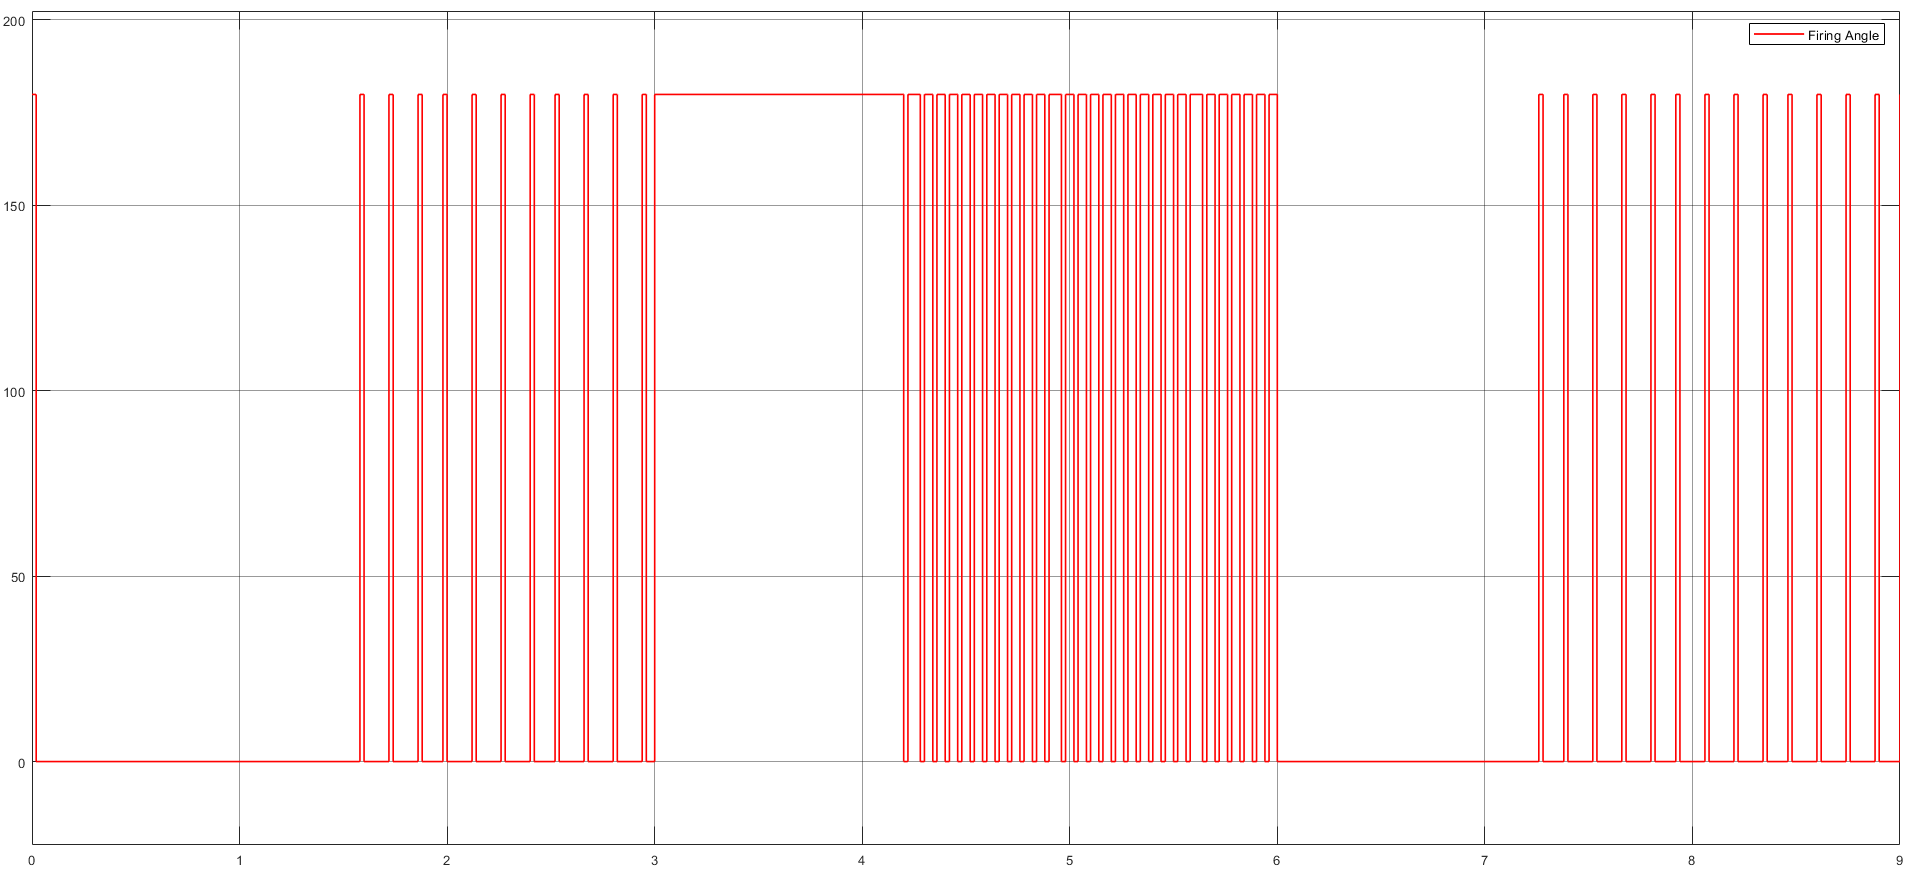
\includegraphics[width=10 cm]{Controller_output_onoff.png}
    \caption{Controller output changes when reference point is changed}
    \label{fig:my_label}
\end{figure}
\subsubsection*{PI Controller}
PI controller is a closed loop feedback mechanism which mostly used industrial applications. By manipulating the error signal, we can abjust time response of a system.
Speed regulation of a DC motor is a type-0 process which has no steady state error when plant driven by PI controller. (System type increased). 
However, the problem is how we closed the loop when we used controlled rectifiers. Since the reference point (speed) and final control element (firing angle) is reversely related we calculate the error signal in following way.   
\begin{figure}[H]
    \centering
    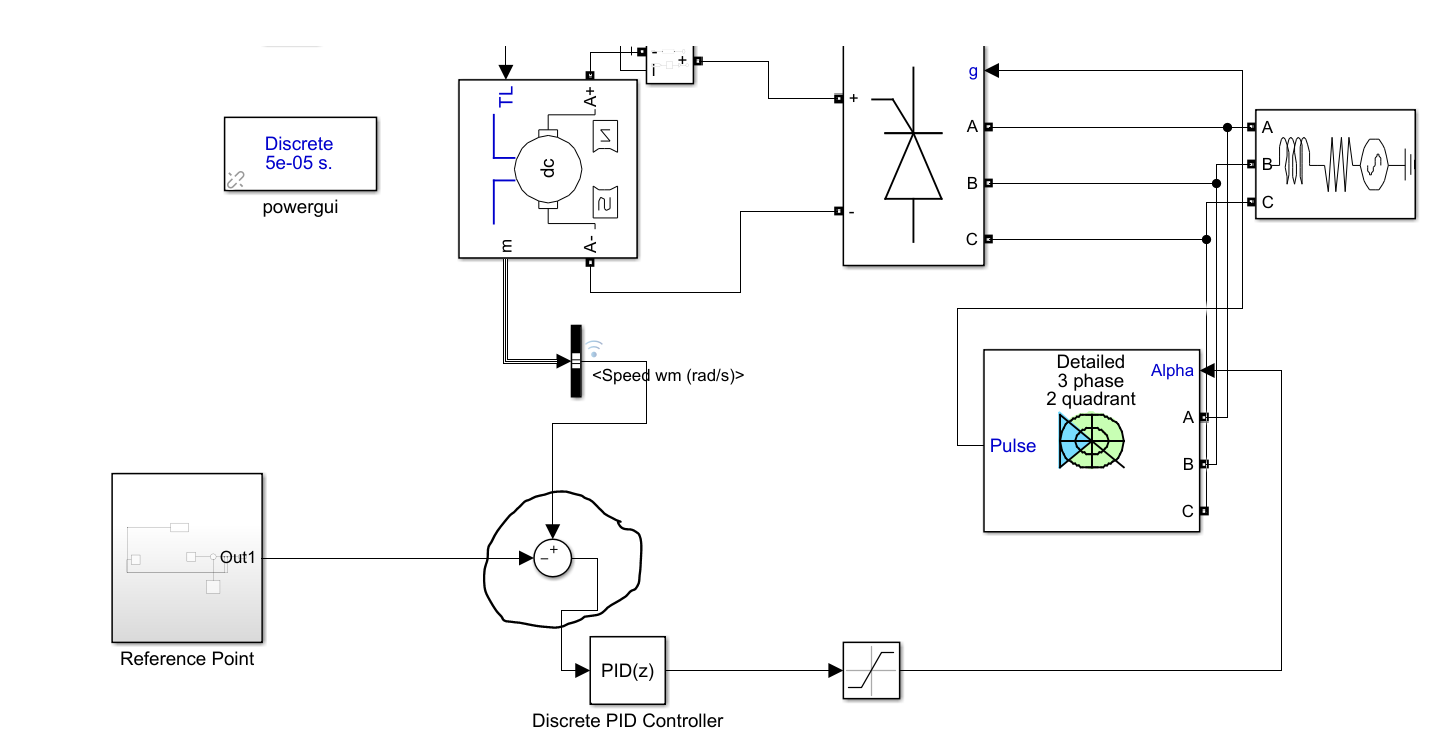
\includegraphics[width=10 cm]{pi_error_signal}
    \caption{The way that we calculate the error signal}
    \label{fig:my_label}
\end{figure}
\begin{figure}[H]
    \centering
    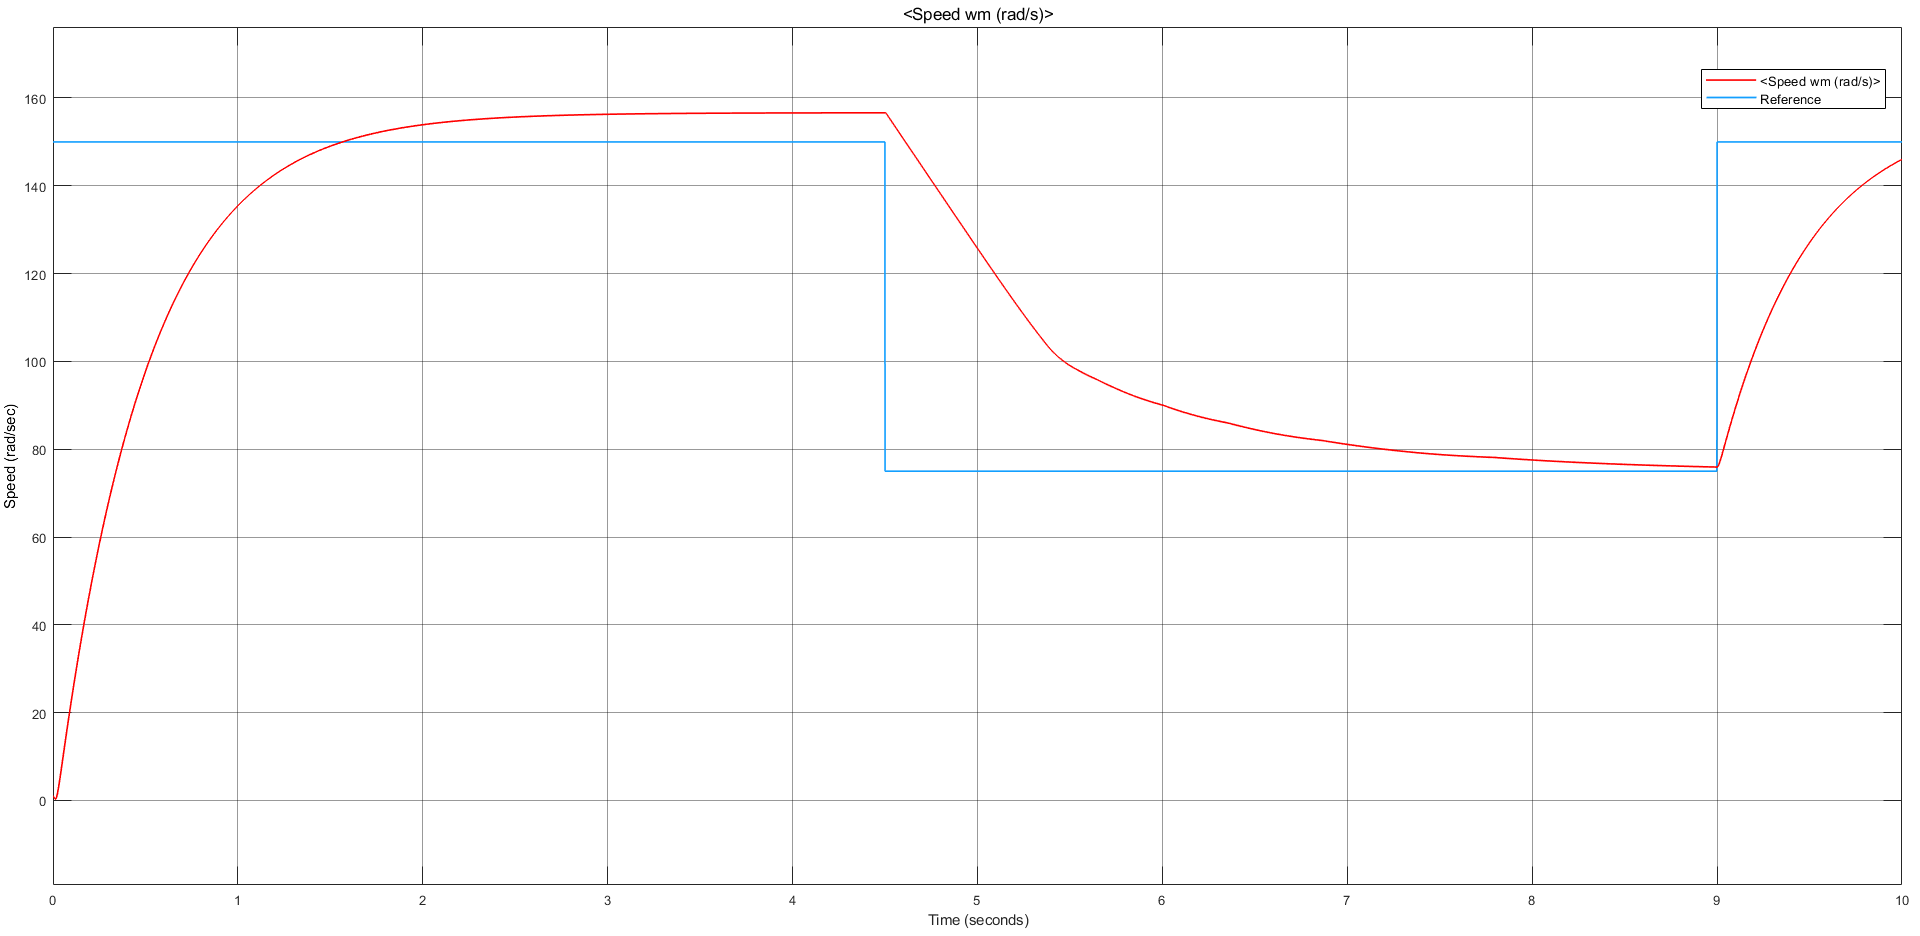
\includegraphics[width=10 cm]{pi_controller_no_extended.png}
    \caption{PI controller time response}
    \label{fig:my_label}
\end{figure}
However we saw nonzero steady state error which we didn't expect. The reason that why this happened is the speed and firing angle relation is not linear. To overcome this problem we come up with the idea of Extended PI Controller.
\subsubsection*{Extended PI Controller}
Since the relation between set point (firing angle) and and control variable (speed of the DC motor) is nonlinear, directly obtaining error function between them has some drawbacks. To indicate these drawbacks first, we should identify the our process. 
\subsubsection{Open loop test}
At this part using Simulink, i collect steady state speed data with various firing angles. Then i transfer the data MATLAB environment to fitting a function for it. 
\subsubsection{Curve Fitting}
Using MATLAB Curve Fitting Toolbox, I formulate the speed and firing angle characteristic by using open loop test results. The final function takes speed as a input and converted to required firing angle.

\begin{figure}[H]%
    \centering
    \subfloat[Simulink Model]{{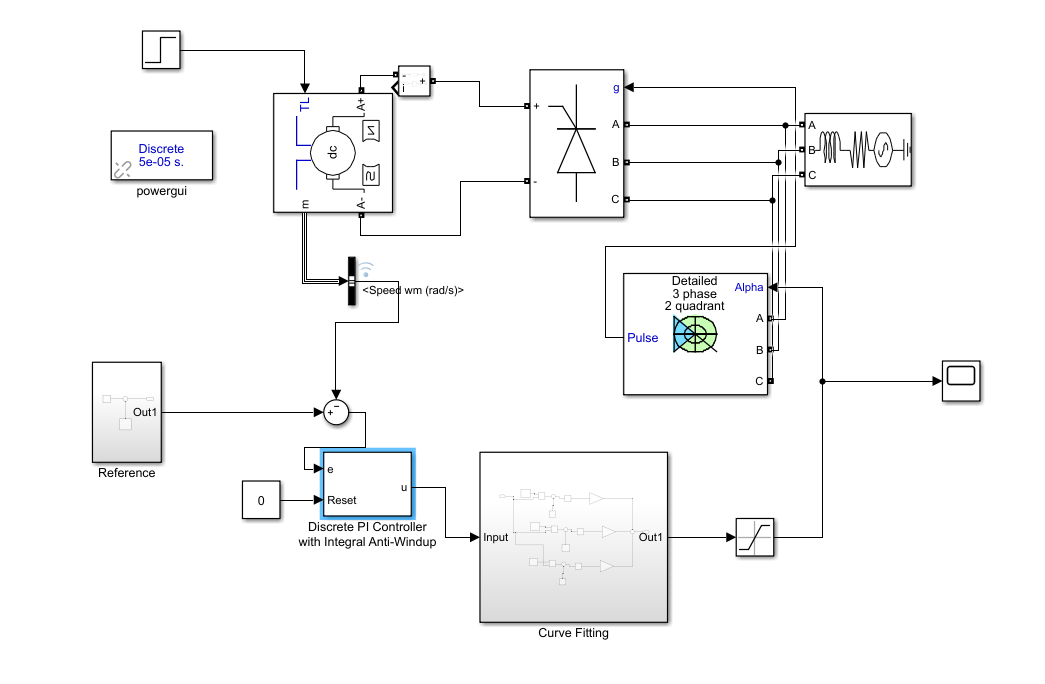
\includegraphics[width=7cm]{extended_pi_controller_simu}}}%
    \qquad
    \subfloat[Speed-firing angle characteristic]{{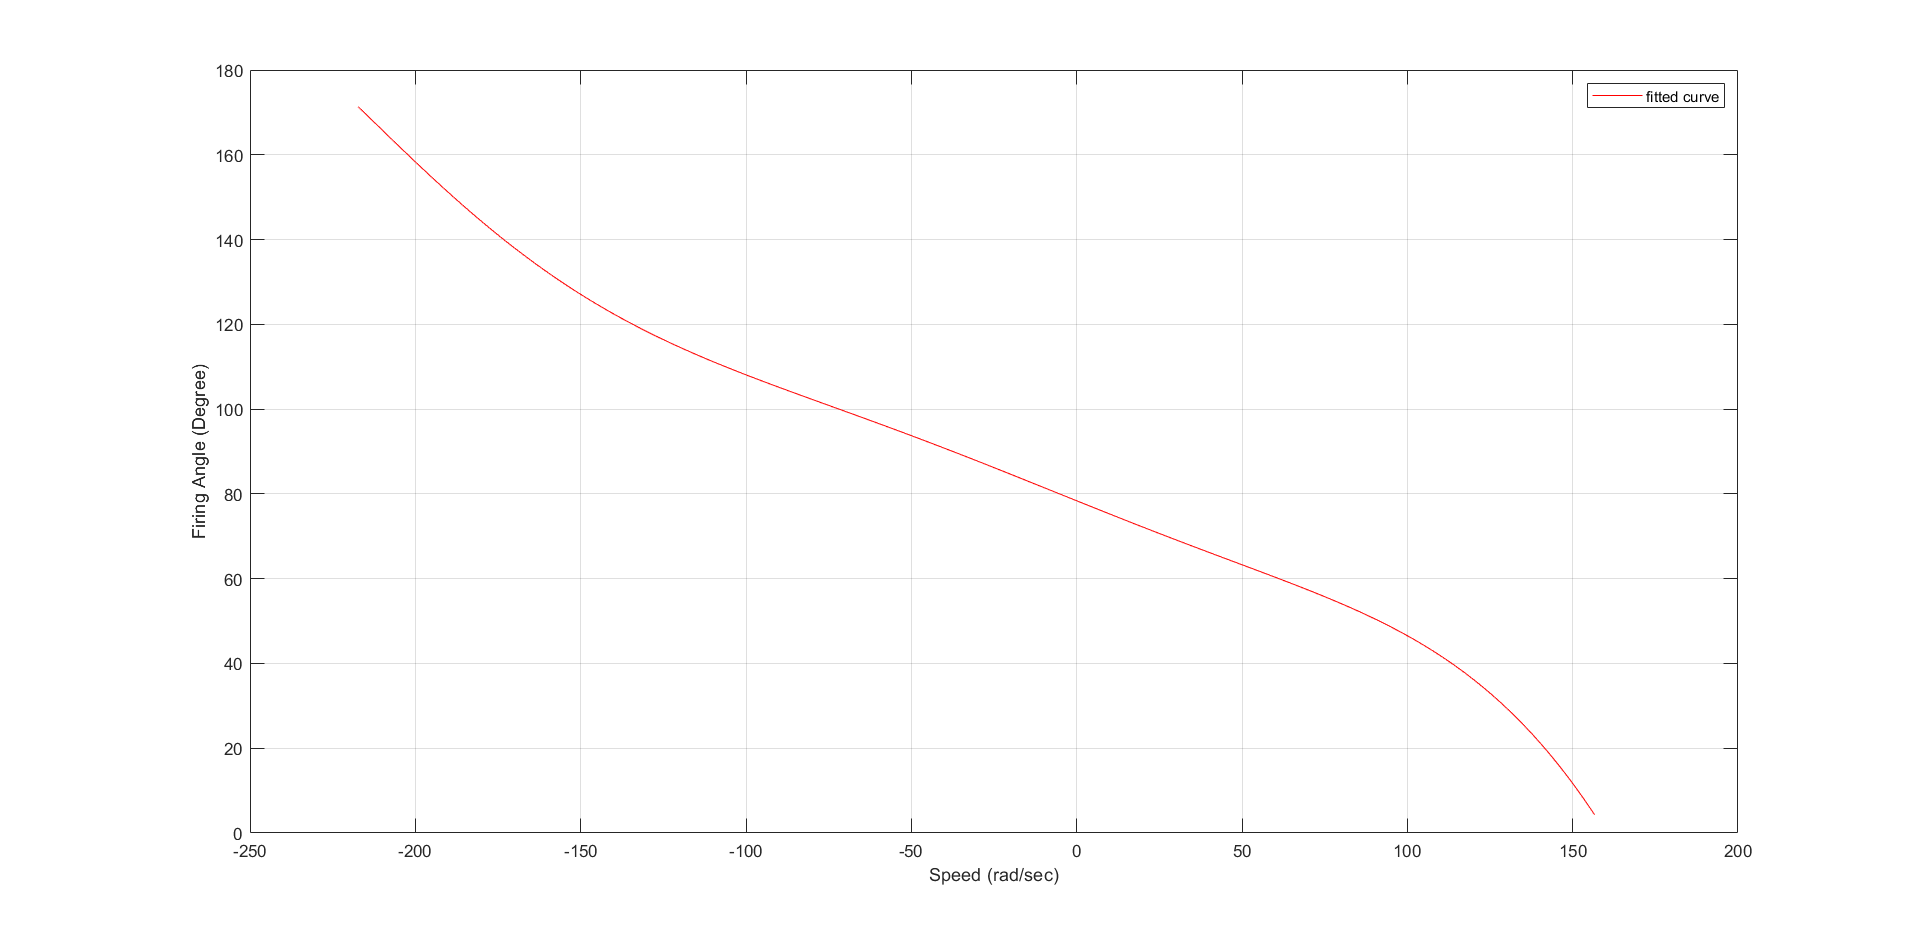
\includegraphics[width=7cm]{function_fitting.png} }}%
    \caption{Speed firing angle relationship}%
    \label{fig:example}%
\end{figure}


\begin{figure}[H]
    \centering
    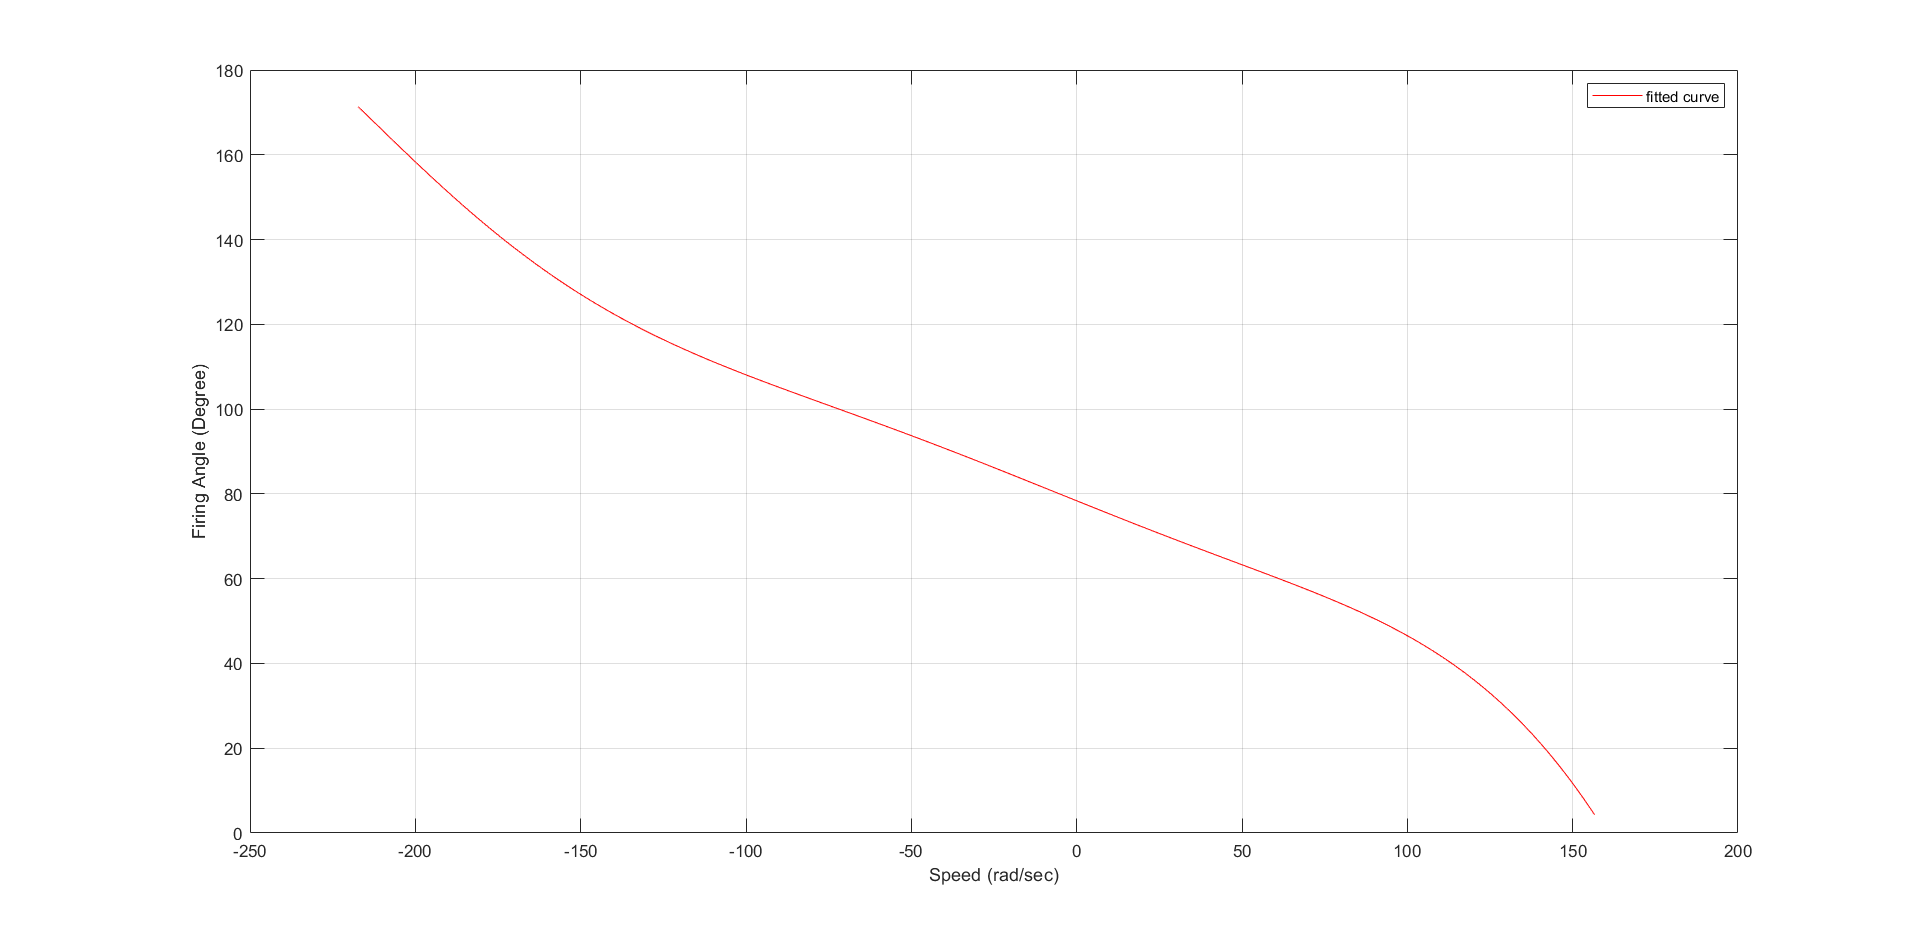
\includegraphics[width=10 cm]{function_fitting.png}
    \caption{Speed-firing angle characteristics}
    \label{fig:my_label}
\end{figure}
\begin{figure}[H]
    \centering
    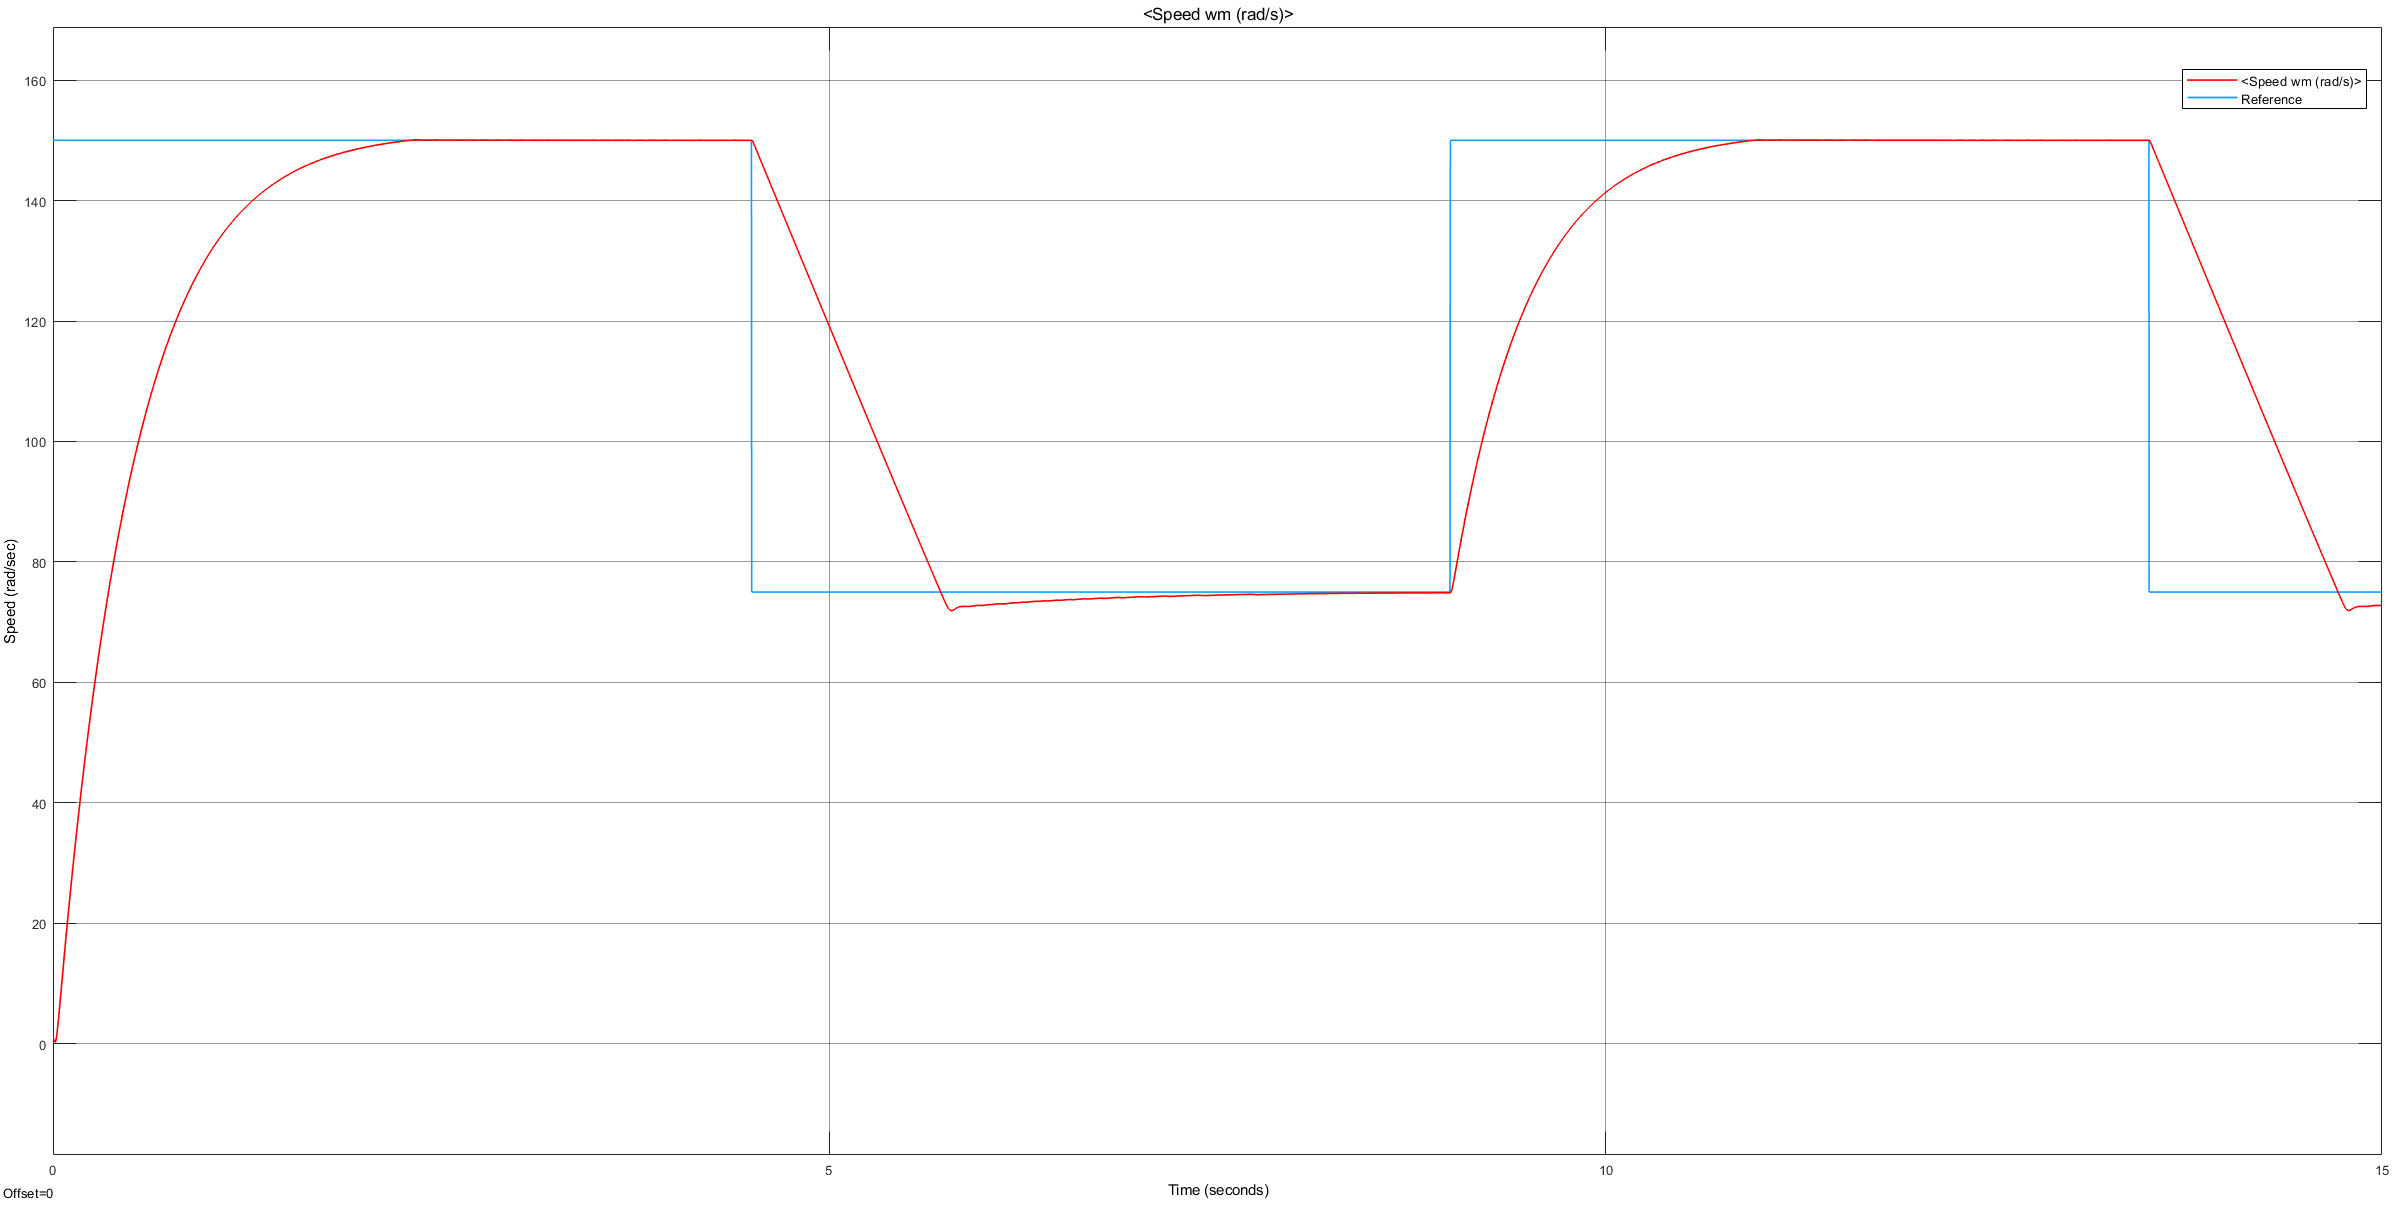
\includegraphics[width=10 cm]{pi_controller.png}
    \caption{Transient performance of extended PI controller}
    \label{fig:my_label}
\end{figure}
Overall motivation of such a PI controller is removing the effect of nonlinearities i.e. steady state error. After using this method we significantly improve steady state error performance without sacrifice system speed. 
\begin{figure}[H]
    \centering
    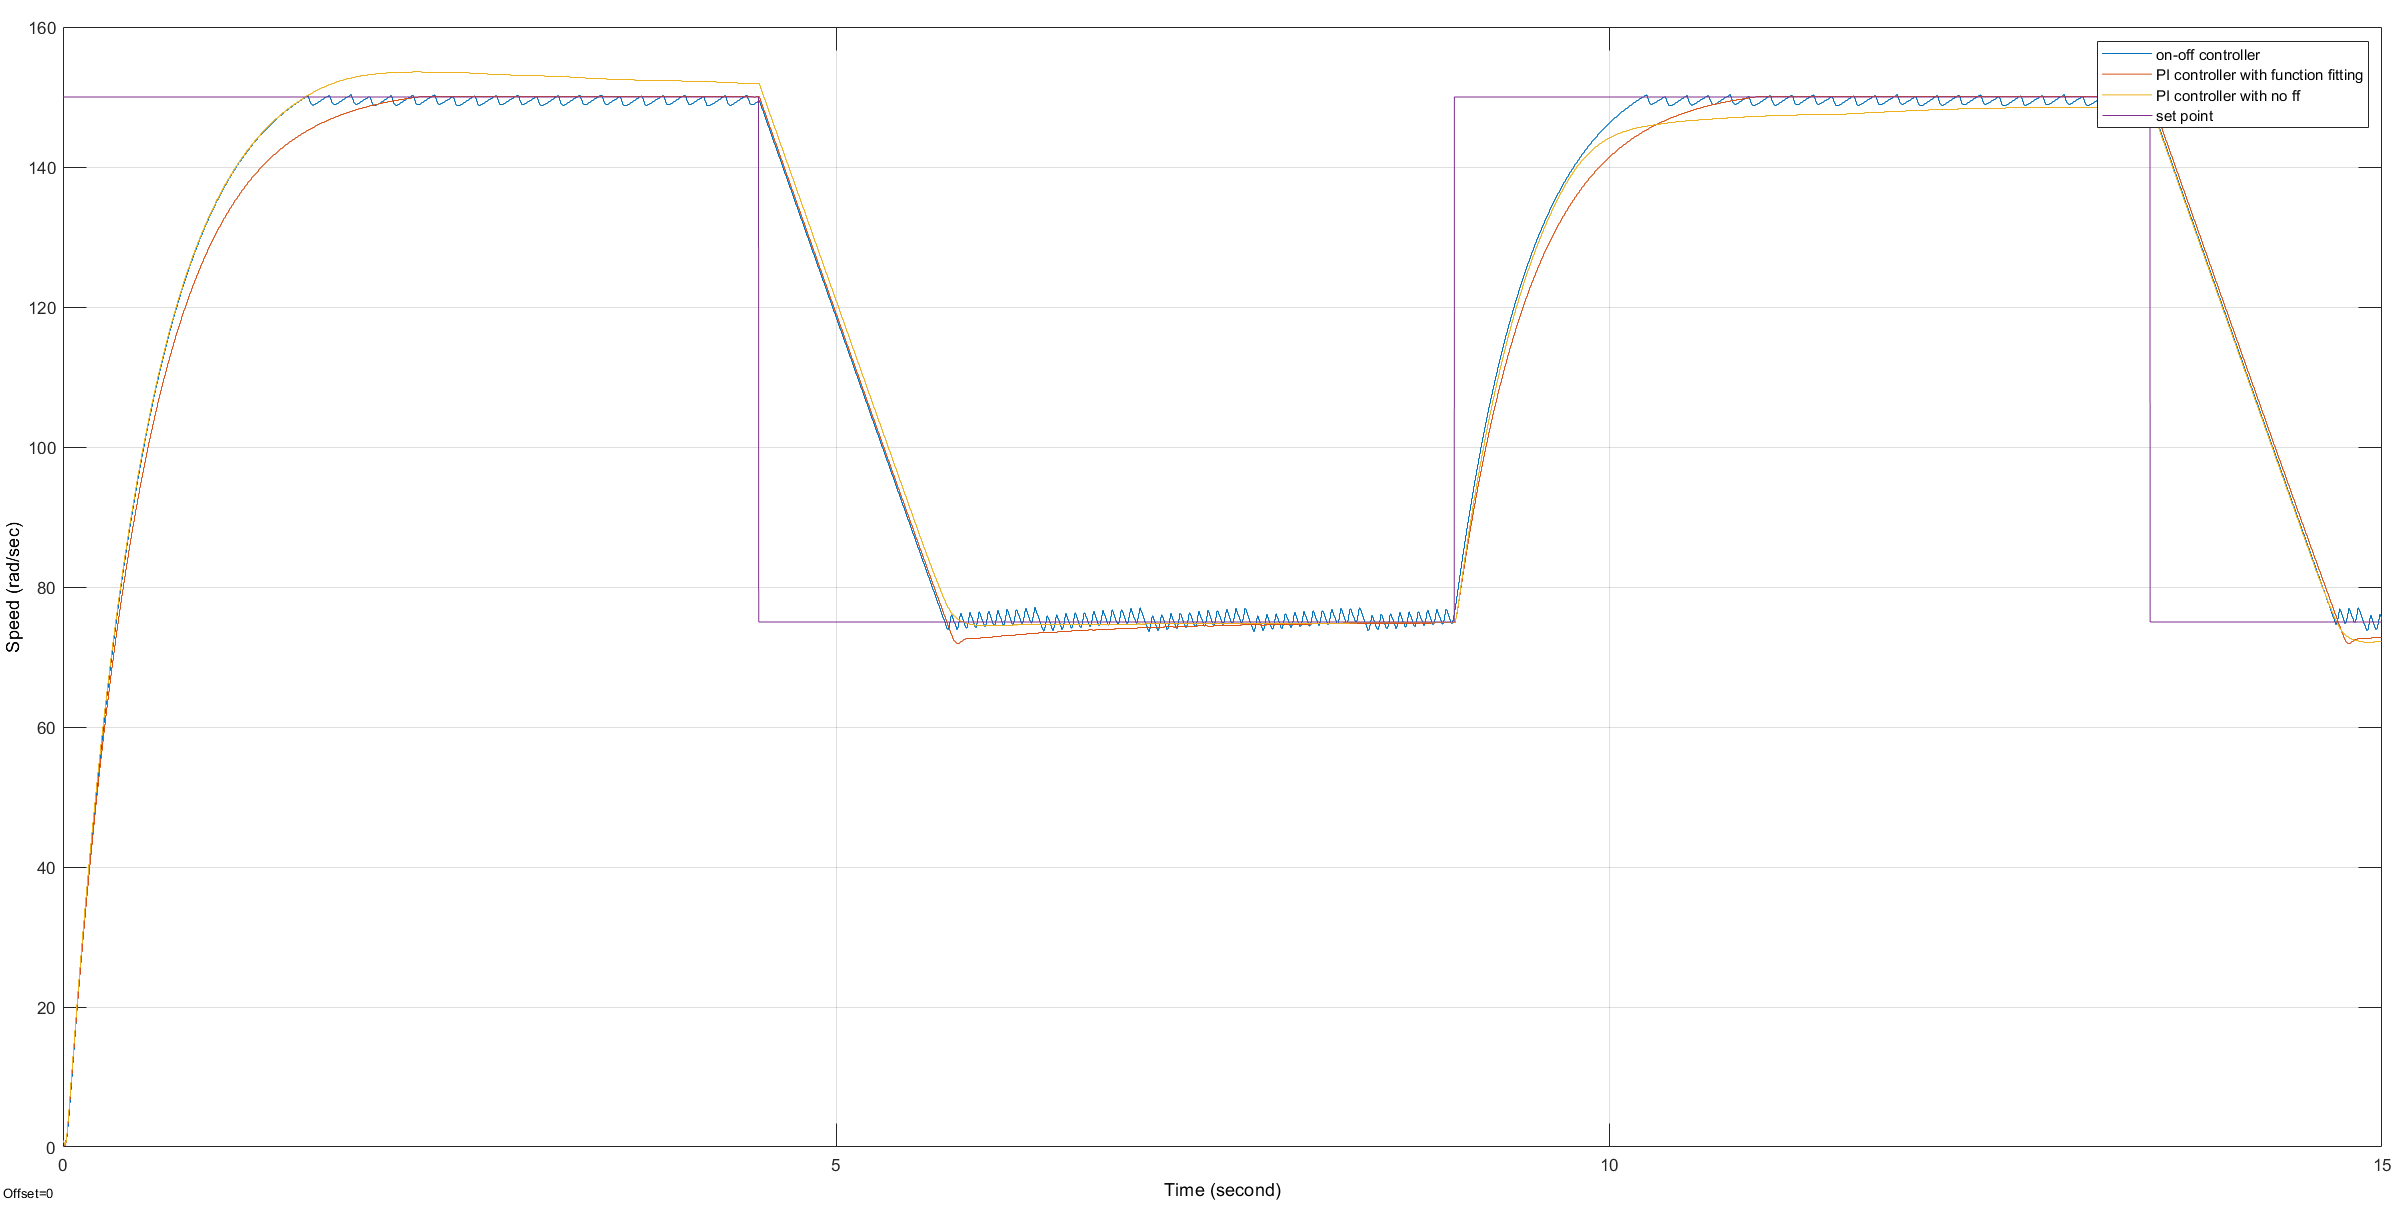
\includegraphics[width=10 cm]{all_controllers.png}
    \caption{Overall comparison of time responses}
    \label{fig:my_label}
\end{figure}
\begin{table}
\begin{tabularx}{\linewidth}{>{\parskip1ex}X@{\kern4\tabcolsep}>{\parskip1ex}X}
\toprule
\hfil\bfseries Pros
&
\hfil\bfseries Cons
\\\cmidrule(r{3\tabcolsep}){1-1}\cmidrule(l{-\tabcolsep}){2-2}

%% PROS, seperated by empty line or \par
It's simple, easy to implement\par
Fast response\par

&

%% CONS, seperated by empty line or \par
Steady state oscillation at output (bang-bang)\par
Aggressive change at semiconductor gate can create extra stress at semiconductor \par


\\\bottomrule
\end{tabularx}
\caption{Pros cons of on-off controller}
\end{table}
\begin{table}
\begin{tabularx}{\linewidth}{>{\parskip1ex}X@{\kern4\tabcolsep}>{\parskip1ex}X}
\toprule
\hfil\bfseries Pros
&
\hfil\bfseries Cons
\\\cmidrule(r{3\tabcolsep}){1-1}\cmidrule(l{-\tabcolsep}){2-2}

%% PROS, seperated by empty line or \par

Great steady state performance (especially at extended version)\par
Controller has flexible, designed response can be obtained by retuning the controller  \par
&

%% CONS, seperated by empty line or \par
Not simple as on-off controller\par
Open loop test must be done for controller calculations\par
Need microcontroller hardware


\\\bottomrule
\end{tabularx}
\caption{Pros cons of PI controller}
\end{table}
\section*{Question 2}

\section*{Question 3}
\end{document}
